\documentclass[a4paper]{llncs}

% Page size (with wide righthand margin, for todo notes)
\usepackage[paperwidth=21cm, paperheight=22cm, textwidth=12.2cm,
textheight=19.3cm]{geometry}
\addtolength\hoffset{-3cm}
\addtolength\marginparwidth{3cm}

% Use Times font (it's more compact)
%\renewcommand\rmdefault{ptm}

% Define a version of \paragraph whose heading runs straight into the
% text that follows.
% {
\makeatletter
\usepackage{suffix}
\renewcommand\paragraph[1]{%
\@startsection{paragraph}{3}{\z@}%
{-12\p@ \@plus -4\p@ \@minus -4\p@}%
{-0.5em \@plus -0.22em \@minus -0.1em}%
{\normalfont\normalsize\bfseries\boldmath}{#1}}
\WithSuffix\newcommand\paragraph*[1]{%
\@startsection{paragraph}{3}{\z@}%
{-12\p@ \@plus -4\p@ \@minus -4\p@}%
{0pt}%
{\normalfont\normalsize\bfseries\boldmath}{#1} \hspace*{0pt}}
\makeatother
%}

% Line numbers in margin
\usepackage{lineno}
\setpagewiselinenumbers
\modulolinenumbers[5]

% Reduce spacing above/below figures
%\setlength\textfloatsep{10.0pt plus 2.0pt minus 4.0pt}
%\setlength\floatsep{6.0pt plus 2.0pt minus 2.0pt}


\usepackage{ifthen}
\usepackage{array}
\usepackage[T1]{fontenc}
\usepackage{url}


% Inline lists
\usepackage[inline]{enumitem}
\newenvironment{inlineitemize}{
\begin{itemize*}[label={},afterlabel={},before=\unskip]
}{
\end{itemize*}
}

% Remove spacing above/below lists
%\setlist{noitemsep, topsep=0pt} 

% Prettier tables
\usepackage{booktabs}

% Multiple footnotes per line
\usepackage[para]{footmisc}

%\usepackage[colorlinks=true,allcolors=blue,breaklinks,draft=false]{hyperref}

\usepackage{amsmath}
%\usepackage{amsthm}
\usepackage{amssymb}
\usepackage{stmaryrd}
\usepackage[usenames,dvipsnames]{xcolor}

% Comments
\usepackage{todonotes}
\setcounter{tocdepth}{1} % Makes \listoftodos work with llncs
\newcommand\JWComment[1]{\todo[backgroundcolor=blue!10,
  linecolor=blue]{{\bf John:} #1}}

% Code listings
\usepackage{listings}
\lstset{
  basicstyle=\small\ttfamily,
  basewidth=0.5em, % when using cmtt
  columns=fixed,
  mathescape=true,
  numberstyle=\scriptsize,
  escapechar=",
  xleftmargin=5mm,
  numbersep=3mm,
}

\usepackage{tikz}
\usetikzlibrary{arrows.meta}
\usetikzlibrary{fit}
\usetikzlibrary{positioning}

% For adding borders/shading to blocks of text
\usepackage{framed}
\definecolor{shadecolor}{gray}{0.9}

% For highlighting text
\usepackage{soul} 
\definecolor{highlightingcolor}{HTML}{FFFF99}
\sethlcolor{highlightingcolor}
\newcommand\mhl[1]{\fboxsep=0pt\colorbox{highlightingcolor}{\strut$#1$}}

\newcommand\stack[2][l]{{\renewcommand\arraystretch{1}\begin{array}[t]{@{}#1@{}}#2\end{array}}}

\newcommand\var[1]{\mathit{#1}}
\newcommand\code[1]{\mbox{\lstinline{#1}}}
\newcommand\sem[1]{\llbracket #1 \rrbracket}
\newcommand\roundsem[1]{\llparenthesis\hspace{0.1ex}#1\hspace{0.1ex}\rrparenthesis}
\newcommand\semicolon{\mathbin{;}}

\title{Dynamic quantifiers and proof graphs}
\author{John Wickerson}
\institute{Imperial College London}

\begin{document}

\maketitle

%\linenumbers

\pagestyle{plain}

\begin{abstract} 
To do.
\end{abstract}

\section{Introduction}

\newcommand\dvd{\mathrel{\var{dvd}}}

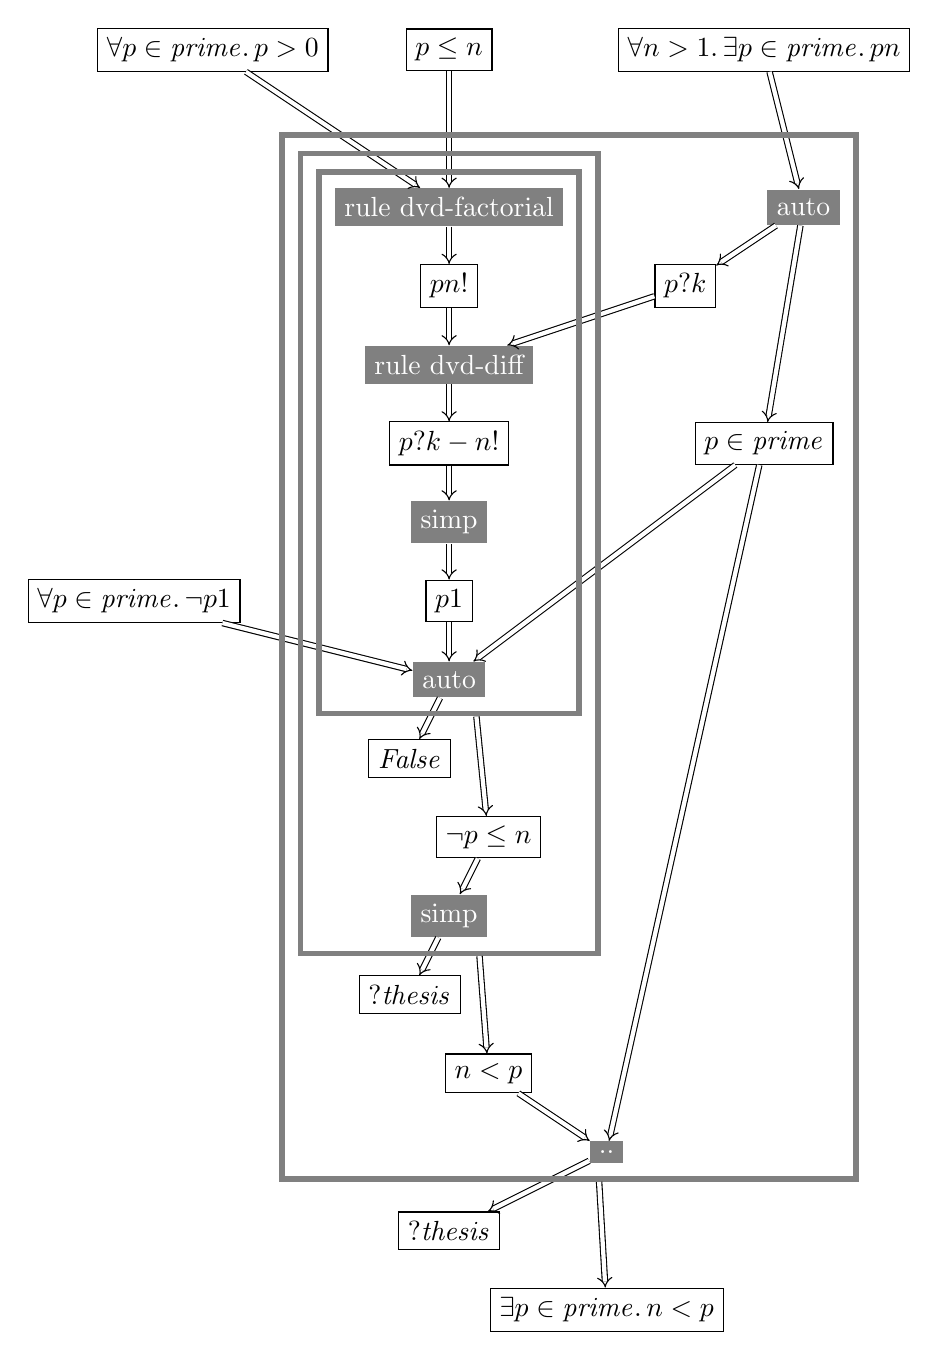
\begin{tikzpicture}[%
  yscale=-1,
  every node/.style={draw,shape=rectangle,black},
  every edge/.style={draw},
  j/.style={text=white,fill=black!50,draw=none},
  f/.style={},
  i/.style={double equal sign distance, -Implies},
  s/.style={inner sep=2mm, line width=2pt, draw=black!50},
]
\node[f] (prime-factor-exists) at (4,2) {$\forall n > 1\ldotp \exists
p \in \var{prime}\ldotp p \dvd n$};
\node[j] (j1) at (4.5,4) {auto};
\node[f] (prime) at (4,7) {$p \in \var{prime}$};
\node[f] (dvd) at (3,5) {$p\dvd {?}k$};
\draw[i] (prime-factor-exists) -- (j1);
\draw[i] (j1) -- (prime);
\draw[i] (j1) -- (dvd);
\node[f] (f3) at (0,2) {$p \le n$};
\node[f] (prime-g-zero) at (-3,2) {$\forall p \in \var{prime}\ldotp p
> 0$};
\node[j] (j2) at (0,4) {rule dvd-factorial};
\node[f] (f4) at (0,5) {$p\dvd n!$};
\draw[i] (f3) -- (j2);
\draw[i] (prime-g-zero) -- (j2);
\draw[i] (j2) -- (f4);
\node[j] (j3) at (0,6) {rule dvd-diff};
\node[f] (f5) at (0,7) {$p\dvd {?}k - n!$};
\draw[i] (f4) -- (j3);
\draw[i] (dvd) -- (j3);
\draw[i] (j3) -- (f5);
\node[j] (j4) at (0,8) {simp};
\node[f] (f6) at (0,9) {$p\dvd 1$};
\draw[i] (f5) -- (j4);
\draw[i] (j4) -- (f6);
\node[f] (prime-nd-one) at (-4,9) {$\forall p \in \var{prime}\ldotp
\neg p \dvd 1$};
\node[j] (j5) at (0,10) {auto};
\node[f] (f7) at (-0.5,11) {$\var{False}$};
\draw[i] (f6) -- (j5);
\draw[i] (prime-nd-one) -- (j5);
\draw[i] (prime) -- (j5);
\draw[i] (j5) -- (f7);
\node[s, fit=(j2) (j3) (j4) (j5)] (s1) {};
\node[f] (f2) at (0.5,12) {$\neg p \le n$};
\draw[i] (s1) -- (f2);
\node[j] (j6) at (0,13) {simp};
\node[f] (f8) at (-0.5,14) {${?}\var{thesis}$};
\draw[i] (f2) -- (j6);
\draw[i] (j6) -- (f8);
\node[s, fit=(s1) (j6)] (s2) {};
\node[f] (f1) at (0.5,15) {$n < p$};
\draw[i] (s2) -- (f1);
\node[j] (j7) at (2,16) {..};
\node[f] (f9) at (0,17) {${?}\var{thesis}$};
\draw[i] (f1) -- (j7);
\draw[i] (prime) -- (j7);
\draw[i] (j7) -- (f9);
\node[s, fit=(j1) (s2) (j7)] (s3) {};
\node[f] (thesis) at (2,18) {$\exists p \in \var{prime}\ldotp n < p$};
\draw[i] (s3) -- (thesis);
\end{tikzpicture}





\bibliographystyle{plain}
\bibliography{dynquants}

%\pagebreak

%\listoftodos


\end{document}

%%% Local Variables:
%%% mode: latex
%%% TeX-master: t
%%% End:
